\documentclass[aspectratio=169]{ctexbeamer}
% \setbeamertemplate{bibliography item}{\insertbiblabel}
\usepackage{booktabs}
\usetheme{Madrid}

\title{Auto-Vectorization \& SIMD in LLVM}
\subtitle{High Performance Computing}

\AtBeginSection[]{
    \begin{frame}
        \vfill
        \centering
        \begin{beamercolorbox}[sep=8pt,center,shadow=true,rounded=true]{title}
            \usebeamerfont{title}\insertsectionhead\par%
        \end{beamercolorbox}
        \vfill
    \end{frame}
}

\beamertemplatenavigationsymbolsempty
\definecolor{tuna}{rgb}{0.098,0.51,0.696}
\definecolor{thu}{rgb}{0.50,0.36,0.71}

\setbeamercolor{section in toc}{fg=black,bg=white}
\setbeamercolor{item}{fg=tuna,bg=white}
\setbeamercolor{alerted text}{fg=tuna!80!gray}
\setbeamercolor*{palette primary}{fg=tuna!60!black,bg=gray!30!white}
\setbeamercolor*{palette secondary}{fg=tuna!70!black,bg=gray!15!white}
\setbeamercolor*{palette tertiary}{bg=tuna!80!black,fg=gray!10!white}
\setbeamercolor*{palette quaternary}{fg=tuna,bg=gray!5!white}

\setbeamercolor*{sidebar}{fg=tuna,bg=gray!15!white}

\setbeamercolor*{palette sidebar primary}{fg=tuna!10!black}
\setbeamercolor*{palette sidebar secondary}{fg=white}
\setbeamercolor*{palette sidebar tertiary}{fg=tuna!50!black}
\setbeamercolor*{palette sidebar quaternary}{fg=gray!10!white}

%\setbeamercolor*{titlelike}{parent=palette primary}
\setbeamercolor{titlelike}{parent=palette primary,fg=tuna}
\setbeamercolor{frametitle}{bg=gray!10!white}
\setbeamercolor{frametitle right}{bg=gray!60!white}

\setbeamercolor*{separation line}{}
\setbeamercolor*{fine separation line}{}

\setbeamertemplate{sections/subsections in toc}[square]
\setbeamertemplate{items}[square]


\author{Y.C. Long}



\begin{document}

\begin{frame}
    \maketitle
\end{frame}

\begin{frame}
    \frametitle{Table of Contents}

    \tableofcontents

\end{frame}

\section{Moore定律的终结和并行化的需求}

\begin{frame}
    \frametitle{Moore's Law to be over}

    集成电路上可容纳的晶体管数目,约每隔两年便会增加一倍

    \begin{figure}[h]
        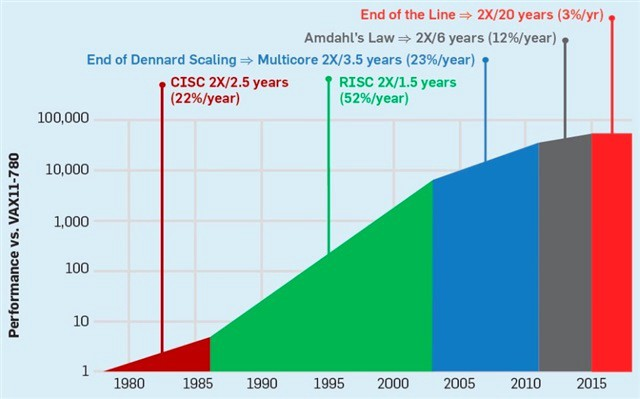
\includegraphics[height=0.5\textheight]{images/moore.jpeg}
        \caption{Moore's Law}
    \end{figure}

\end{frame}

\begin{frame}
    \frametitle{Parallel}

    提高计算机性能的方法,是并行化。

    \begin{figure}[h]
        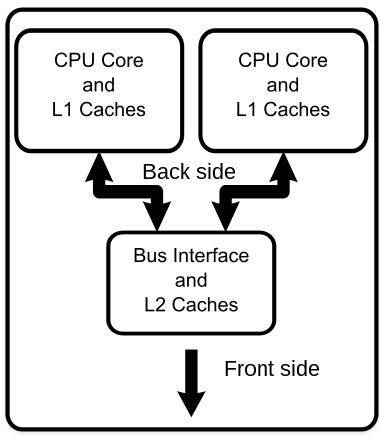
\includegraphics[height=0.5\textheight]{images/dual_core.png}
        \caption{Dual Core Cache Design}
    \end{figure}

\end{frame}

\section{并行的手段}

\subsection{Multi-Core}

\begin{frame}
    \frametitle{Multi-Core}

    为了实现并行化,我们可以给一个计算机加入多个核心。

    \begin{itemize}
        \item 不同的寄存器
        \item 不同的中断处理请求
        \item 操作系统-对称多处理(SMP)调度
    \end{itemize}

    \begin{figure}[h]
        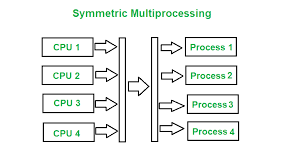
\includegraphics[height=0.45\textheight]{images/smp.png}
        \caption{Symmetric multiprocessing}
    \end{figure}

\end{frame}

\subsection{Single-Core}

\begin{frame}
    \frametitle{Single-Core - Out-of-Order Execution}

    乱序执行(Out-of-Order Execution)是现代CPU最基本的一个并行手段。

    % TODO: 展示乱序执行的例子

\end{frame}

\begin{frame}
    \frametitle{Single-Core - SIMD}

    OoOE在编程上由编译器全局指令调度器(Instruction Scheduler)优化。

    单指令流多数据流(Single instruction, multiple data (SIMD)),提供了一种让我
    们更好地进行向量计算的方式。

    % TODO: SIMD graph

\end{frame}

\begin{frame}
    \frametitle{Benefits of SIMD}

    通常情况下我们很难将串行代码转化为并行,为了设计并行算法通常需要改变原有的
    逻辑。

    \begin{figure}[h]
        \centering
        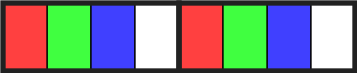
\includegraphics[width=0.5\textwidth]{images/rgba.png}
        \caption{RGBA}
    \end{figure}

    如图所示,在图形学中我们经常需要计算图像的颜色信息,而颜色在RGBA几个维度下
    的计算是可以向量化的。

\end{frame}


\begin{frame}
    \frametitle{GPGPU}

    显卡(GPU)包含大量的核心来支持高度并行化的计算,最开始的在显卡上的编程是很困
    难的,随着时代的发展显卡的计算能力越来越不容小觑,通用计算显卡(GPGPU)也开始
    包含在编译优化的领域。如何把科研大佬写的模型,放到真正的显卡上执行?

    \begin{figure}[h]
        \centering
        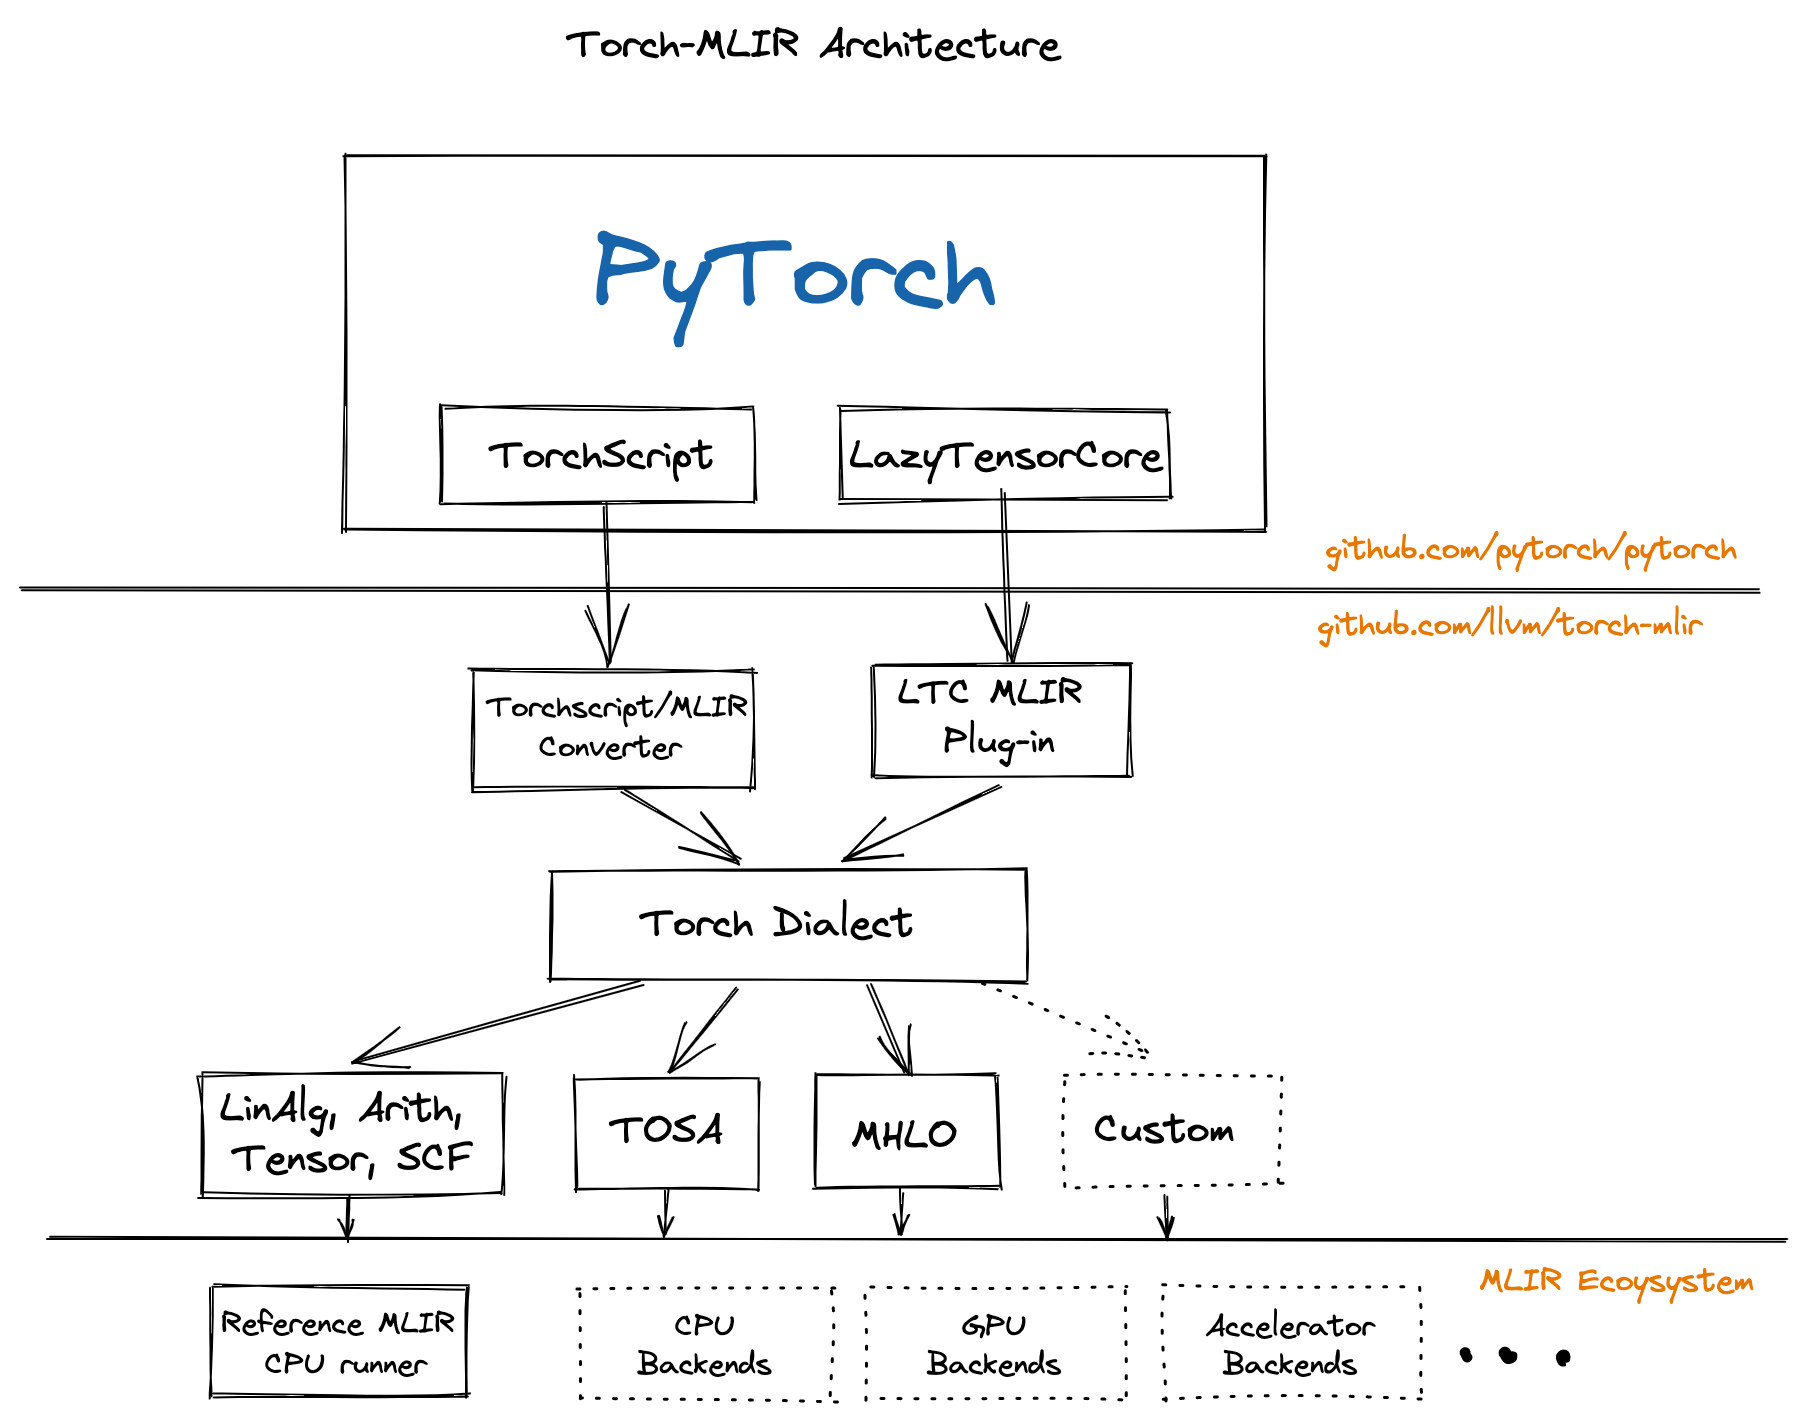
\includegraphics[height=0.5\textheight]{images/torch-mlir.png}
        \caption{Torch-MLIR}
    \end{figure}

\end{frame}

\begin{frame}
    \frametitle{Problem With SIMD Instructions}

    \begin{block}{RISC-V Designers}
        \textit{SIMD Instructions considered harmful. -- David Patterson}
    \end{block}

    一开始,SIMD被认为是实现并行化简单有效的方法。我们将64位寄存器和ALU划分为许
    多8, 16, 32位的块,然后并行地计算它们。用每条指令的操作码(opcode)提供数据宽
    度和操作。

    \textbf{指令集膨胀}

    IA-32指令集已经从最开始的80多条指令增长到了现在的1400多条。SSE, AVX, 各种
    SIMD扩展和宽寄存器让指令集变得越来越复杂。
\end{frame}

\end{document}
